\documentclass[12pt]{article}

\usepackage{enumitem}
\usepackage{titling}

\usepackage[utf8]{inputenc}
\usepackage[T1]{fontenc}
\usepackage{fvextra}
\usepackage[spanish]{babel}
\usepackage{geometry}
\usepackage{hyperref}
\hypersetup{hidelinks}
\usepackage{fancyhdr}
\usepackage{listings}
\usepackage{listingsutf8}
\usepackage{graphicx}
\usepackage{eso-pic} % Para insertar imágenes de fondo en páginas específicas
\usepackage{xcolor}
\usepackage{transparent}

% Encabezado y pie de página
\pagestyle{fancy}
\fancyhf{}
\lhead{Curso de Introducción a la IA para Personas Mayores}
\rhead{\thepage}
\cfoot{Preparado por el Centro de Mayores (Ciberaula)}

\title{\Huge Curso Introductorio de Inteligencia Artificial\\ \Large Para Personas Mayores}
\author{Centro de Mayores (Ciberaula)}
\date{1 de abril de 2025\\San Fernando de Henares}

\begin{document}
\newcommand\portada{
	\thispagestyle{empty}
	\AddToShipoutPictureBG*{
		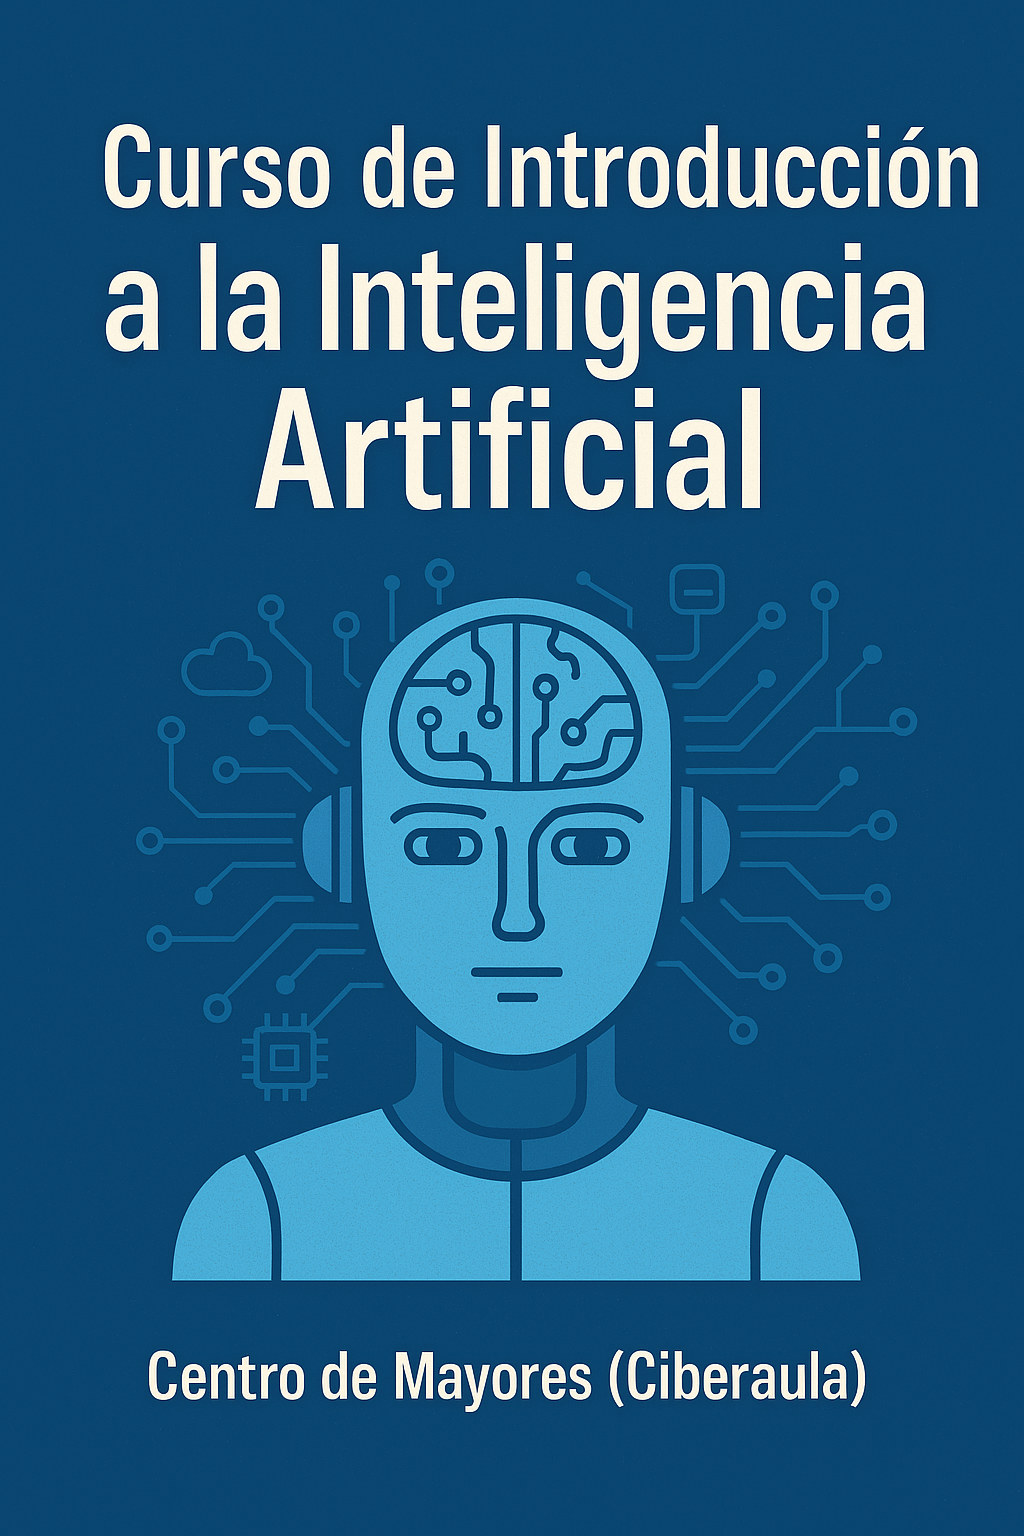
\includegraphics[width=\paperwidth,height=\paperheight]{Portada_Curso02.png}
	}
	\null
	\newpage
}
\portada
	
	% Carátula
%	\begin{titlepage}
%		\centering
%		\vspace*{2cm}
%		{\Huge \textbf{Curso Introductorio de Inteligencia Artificial}}\\[1.5ex]
%		{\LARGE Para Personas Mayores}\\[4ex]
%		% Ajusta el nombre de la imagen si dispones de ella.
%		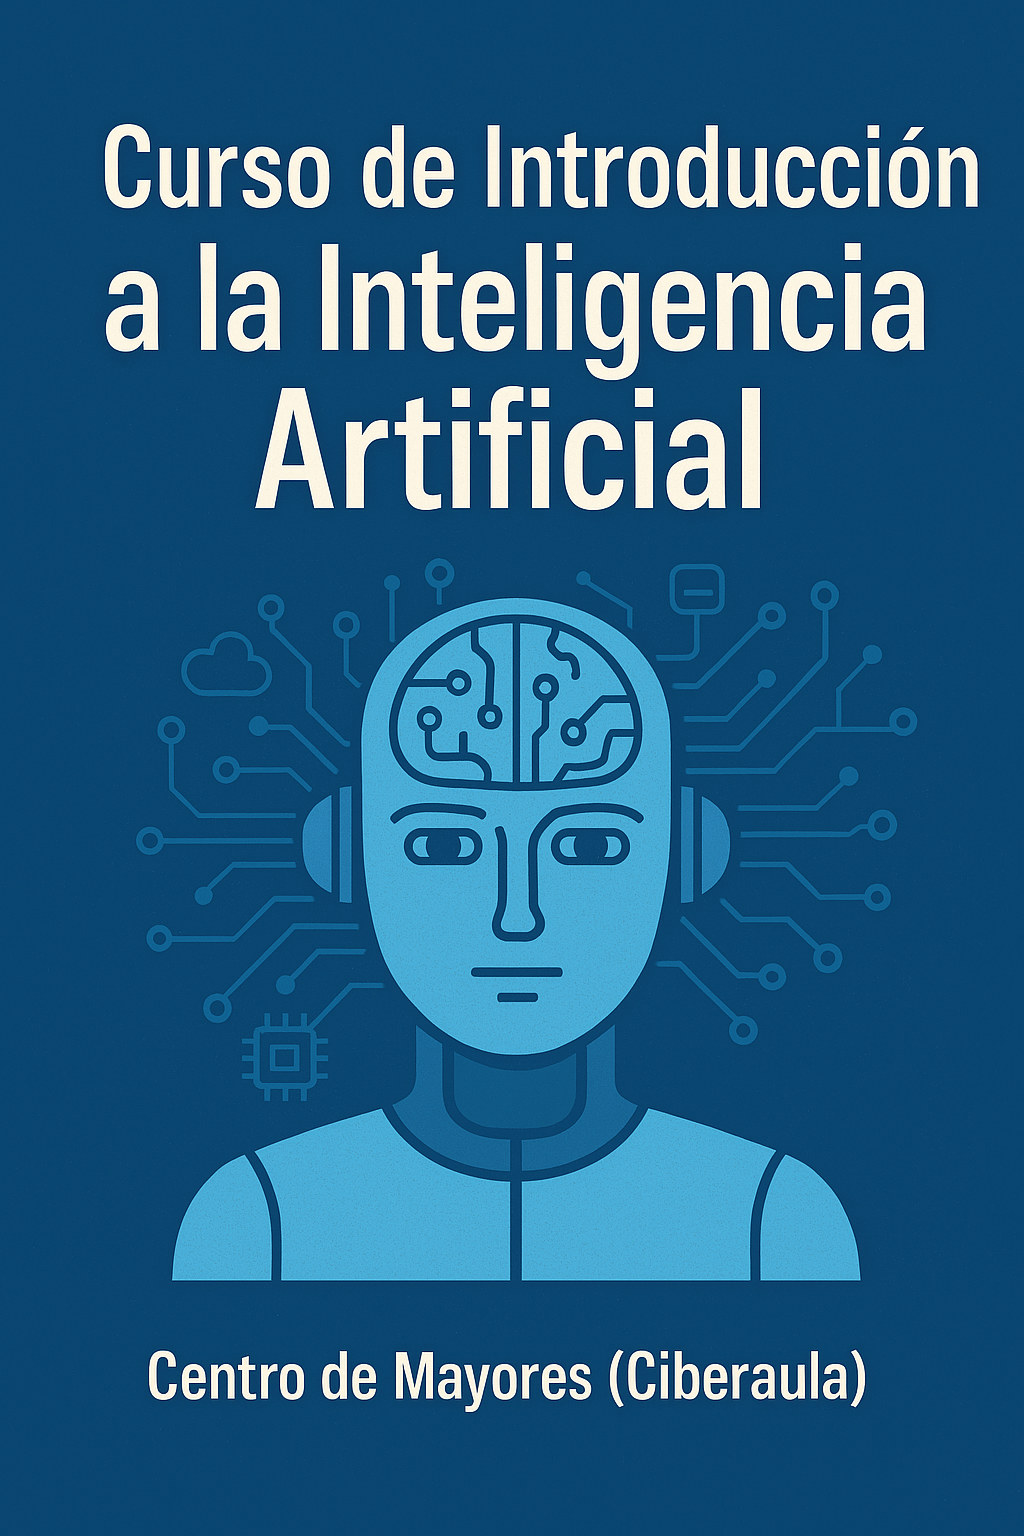
\includegraphics[width=0.7\textwidth]{Portada_Curso02.png}\\[4ex]
%		\textbf{Preparado por:}\\ Centro de Mayores (Ciberaula)\\[2ex]
%		\textbf{Fecha:}\\ 1 de abril de 2025\\[4ex]
%		\vfill
%		\textit{“Aprender nunca envejece”}
%	\end{titlepage}
	
	% Contraportada
	\newpage
	~
	\thispagestyle{empty}
	\vspace*{2cm}
	\begin{center}
		\textbf{\Large Curso Introductorio de Inteligencia Artificial}\\[1ex]
		\textbf{Para Personas Mayores}\\[4ex]
	\end{center}
	
	\noindent Este curso está diseñado para acercar el fascinante mundo de la inteligencia artificial a las personas mayores, explicando de forma clara y amigable qué es, cómo nos afecta y cómo podemos utilizarla para nuestro bienestar diario.
	
	\vspace{1cm}
	\textbf{¿A quién va dirigido?}\\
	Personas mayores interesadas en aprender sobre tecnología, independientemente de su nivel previo de conocimientos.
	
	\vspace{0.5cm}
	\textbf{Objetivos del curso:}
	\begin{itemize}
		\item Comprender los conceptos básicos de la IA.
		\item Descubrir aplicaciones útiles y cotidianas.
		\item Desarrollar criterio y confianza en el uso de herramientas digitales.
		\item Fomentar la reflexión y el debate sobre los cambios tecnológicos.
	\end{itemize}
	
	\vspace{0.5cm}
	\textbf{Autor:} Centro de Mayores (Ciberaula)\\
	\textbf{San Fernando de Henares, 2025}
	
	\vfill
	\begin{center}
		\textit{“Nunca es tarde para aprender algo nuevo”}
	\end{center}
	
	\newpage
	
	\tableofcontents
	\newpage
	
	\section*{Introducción}
	La inteligencia artificial (IA) ya forma parte de nuestra vida diaria, aunque muchas veces no seamos conscientes de ello. Este curso está diseñado especialmente para personas mayores, con explicaciones sencillas, muchos ejemplos y sin necesidad de conocimientos previos de informática. Nuestro objetivo es comprender, sin miedo, qué es la IA, cómo nos afecta y cómo podemos usarla para mejorar nuestra vida cotidiana.
	
	\section{\textbf{\normalsize Módulo 1: Introducción a la Inteligencia Artificial}}
	
	\subsection*{¿Qué es la inteligencia artificial?}
	La inteligencia artificial es la capacidad que tienen algunas máquinas o programas informáticos para realizar tareas que, normalmente, requieren inteligencia humana. Por ejemplo, entender el lenguaje, reconocer una cara, tomar decisiones o aprender de la experiencia.
	
	\textbf{Ejemplo}: Cuando usamos el teléfono móvil para hablar con un asistente como Siri o Google, estamos usando inteligencia artificial. El sistema “entiende” lo que decimos y nos responde con información.
	
	\subsection*{Diferencias entre inteligencia humana e inteligencia artificial}
	\begin{itemize}
		\item La inteligencia humana tiene emociones, creatividad y conciencia. Puede razonar más allá de lo aprendido.
		\item La inteligencia artificial aprende de datos y patrones, pero no tiene sentimientos ni conciencia. Solo actúa según lo que se le ha enseñado.
	\end{itemize}
	
	\textbf{Ejemplo}: Un humano puede crear una poesía desde sus emociones; una IA puede imitar un poema analizando muchos ejemplos anteriores.
	
	\subsection*{Breve historia de la IA}
	\begin{itemize}
		\item \textbf{1950s}: Alan Turing plantea si las máquinas pueden pensar.
		\item \textbf{1960s-70s}: Primeros programas que resolvían problemas lógicos.
		\item \textbf{1980s}: Se crean los “sistemas expertos” usados en medicina y otras áreas.
		\item \textbf{2000s en adelante}: La IA se expande con internet, teléfonos inteligentes y grandes cantidades de datos.
	\end{itemize}
	
	\subsection*{¿Dónde está presente la IA hoy en día?}
	\begin{itemize}
		\item En los teléfonos móviles (asistentes, cámaras inteligentes)
		\item En los buscadores de internet (Google, Bing)
		\item En la televisión (recomendaciones de series y películas)
		\item En los coches (ayudas al aparcamiento o conducción asistida)
		\item En la medicina (diagnóstico por imagen, seguimiento de pacientes)
		\item \textbf{Otras aplicaciones comunes (en desarrollo)}: Chatbots para atención al cliente, robots que ayudan en el hogar, asistentes de lectura para personas con problemas de visión, análisis de cultivos en la agricultura, vigilancia inteligente, generación automática de noticias o resúmenes, y herramientas creativas para escribir textos, componer música o generar imágenes.
	\end{itemize}
	
	\textbf{Ejemplo}: Cuando Netflix nos recomienda una película que podría gustarnos, lo hace usando IA que ha aprendido de nuestras elecciones anteriores.
	
	\newpage
	
	\section{\textbf{\normalsize Módulo 2: La IA en la vida cotidiana}}
	
	\subsection*{Asistentes de voz: Siri, Alexa y Google Assistant}
	Los asistentes de voz permiten hablarle al teléfono o a dispositivos inteligentes para pedir ayuda o realizar tareas. Se utilizan cada vez más por su comodidad.
	
	\textbf{Ejemplo}: Podemos decir “¿Qué tiempo hace hoy?” o “Recuérdame tomar la pastilla a las 10” y el asistente lo entiende y responde.
	
	\subsection*{Recomendaciones personalizadas: Netflix, YouTube, Amazon}
	La IA analiza nuestros gustos y comportamientos para sugerirnos contenidos o productos.
	\begin{itemize}
		\item En Netflix: sugiere películas similares a las que hemos visto.
		\item En YouTube: recomienda vídeos que podrían interesarnos.
		\item En Amazon: propone productos basados en compras anteriores.
	\end{itemize}
	
	\textbf{Ejemplo}: Si vemos muchos documentales de naturaleza, Netflix tenderá a mostrarnos más de ese estilo.
	
	\subsection*{Móviles y cámaras inteligentes}
	Los teléfonos modernos usan IA para mejorar fotos, detectar rostros, traducir texto con la cámara y sugerir respuestas automáticas.
	
	\textbf{Ejemplo}: Cuando tomamos una foto, el móvil puede mejorarla automáticamente ajustando la luz y el color.
	
	\subsection*{Traductores automáticos y subtítulos en tiempo real}
	La IA permite traducir frases habladas o escritas en diferentes idiomas casi al instante. También genera subtítulos cuando alguien habla.
	
	\textbf{Ejemplo}: Podemos usar Google Translate para hablar en otro idioma con alguien durante un viaje.
	
	\subsection*{Aplicaciones útiles para personas mayores}
	\begin{itemize}
		\item Recordatorios de medicación y citas.
		\item Seguimiento de actividad física o sueño.
		\item Asistentes visuales para leer textos pequeños.
		\item Aplicaciones para llamar a familiares con solo pulsar un botón.
	\end{itemize}
	
	\textbf{Ejemplo}: Una app puede avisarnos todos los días a la misma hora que es momento de tomar una pastilla.
	
	\newpage
	
	\section{\textbf{\normalsize Módulo 3: Cómo funciona la IA sin tecnicismos}}
	
	\subsection*{¿Qué significa aprender para una máquina?}
	Aprender para una máquina significa que puede mejorar su comportamiento a partir de la experiencia, sin que alguien le diga exactamente qué hacer en cada situación. Esto se llama “aprendizaje automático” o “machine learning”.
	
	\textbf{Ejemplo}: Si una IA ve muchas fotos de gatos y perros y se le dice cuáles son cuáles, podrá aprender a diferenciarlos sola cuando vea una nueva imagen.
	
	\subsection*{Ejemplo simple: reconocer entre gatos y perros}
	Imaginemos que queremos que una IA reconozca si una imagen es de un gato o de un perro. El proceso sería así:
	\begin{enumerate}
		\item Le mostramos muchas imágenes de gatos y perros.
		\item A cada imagen le indicamos si es un gato o un perro.
		\item La IA analiza las diferencias (por ejemplo, forma de las orejas, tamaño del hocico).
		\item Cuando vea una imagen nueva, intentará adivinar si es gato o perro basándose en lo que ha aprendido.
	\end{enumerate}
	
	\subsection*{Diferencia entre programar y enseñar}
	\begin{itemize}
		\item Programar es decirle a la máquina exactamente qué hacer en cada paso.
		\item Enseñar es darle ejemplos para que ella misma aprenda las reglas.
	\end{itemize}
	
	\textbf{Ejemplo}: En lugar de decirle a la máquina “si tiene orejas largas y hocico corto es un perro”, simplemente le mostramos muchas fotos y ella deduce esa regla sola.
	
	\subsection*{Lo que una IA no puede hacer (todavía)}
	\begin{itemize}
		\item No puede tener emociones reales ni conciencia.
		\item No entiende el mundo como lo hace una persona.
		\item Puede cometer errores si los datos que ha aprendido son incorrectos o insuficientes.
		\item No tiene sentido común: puede dar respuestas absurdas si no entiende bien el contexto.
	\end{itemize}
	
	\textbf{Ejemplo}: Una IA puede reconocer una cara, pero no sabe si la persona está contenta o triste a menos que se lo hayamos enseñado específicamente.
	
	\newpage
	
	\section{\textbf{\normalsize Módulo 4: Ventajas y riesgos de la IA}}
	
	\subsection*{Beneficios de la inteligencia artificial}
	La IA puede ser una gran ayuda para mejorar la calidad de vida, especialmente para personas mayores. Algunos de sus beneficios más importantes son:
	\begin{itemize}
		\item \textbf{Salud}: control de enfermedades, recordatorios de medicación, asistencia médica remota.
		\item \textbf{Seguridad}: cámaras inteligentes que detectan movimientos extraños, sensores de caída.
		\item \textbf{Comodidad}: automatización del hogar, asistentes que responden por voz, recomendaciones útiles.
		\item \textbf{Acompañamiento}: programas que conversan, leen noticias o ayudan a ejercitar la mente.
	\end{itemize}
	
	\textbf{Ejemplo}: Un reloj inteligente puede medir el pulso, contar los pasos y avisar si detecta una posible caída.
	
	\subsection*{Riesgos: privacidad, fraudes, uso indebido}
	Aunque útil, la IA también presenta algunos peligros que debemos conocer:
	\begin{itemize}
		\item \textbf{Privacidad}: algunas aplicaciones recopilan mucha información personal.
		\item \textbf{Fraudes}: se pueden usar voces falsas o mensajes automáticos para engañar.
		\item \textbf{Uso indebido}: la IA puede ser mal utilizada por empresas o gobiernos sin el consentimiento del usuario.
	\end{itemize}
	
	\textbf{Ejemplo}: Un anuncio que parece personalizado puede haber sido generado tras analizar nuestros gustos sin que lo supiéramos.
	
	\subsection*{Falsificaciones con IA: imágenes y vídeos falsos}
	Hoy en día es posible crear imágenes, audios o vídeos falsos que parecen reales. A esto se le llama \textit{deepfake} y puede confundir fácilmente a cualquiera.
	
	\textbf{Ejemplo}: Se puede crear un vídeo donde una persona diga algo que nunca dijo, usando su imagen y su voz.
	
	\subsection*{Consejos para protegerse y actuar con sentido común}
	\begin{itemize}
		\item No compartir información personal en redes sociales o sitios que no conozcamos.
		\item Desconfiar de mensajes que pidan dinero, contraseñas o datos urgentes.
		\item Verificar la fuente de una noticia o vídeo antes de creerlo o compartirlo.
		\item Pedir ayuda a familiares o personas de confianza si se recibe algo sospechoso.
	\end{itemize}
	
	\textbf{Recuerda}: la mejor protección es la información. Entender cómo funciona la tecnología nos permite usarla con más seguridad y confianza.
	
	\newpage
	
	\section{\textbf{\normalsize Módulo 5: IA con ética y responsabilidad}}
	
	\subsection*{¿Puede la IA tomar decisiones justas?}
	La inteligencia artificial puede ayudar en la toma de decisiones, pero no siempre es justa. Todo depende de los datos con los que ha sido entrenada. Si los datos están incompletos o son injustos, la IA también lo será.
	
	\textbf{Ejemplo}: Si una IA aprende a seleccionar candidatos para un trabajo usando datos históricos donde se prefería a hombres, podría repetir esa injusticia sin querer.
	
	\subsection*{¿Quién es responsable de lo que hace una IA?}
	Aunque una IA tome decisiones, la responsabilidad sigue siendo de los seres humanos que la diseñan, programan o utilizan.
	\begin{itemize}
		\item Las empresas deben garantizar que sus sistemas no hagan daño ni discriminen.
		\item Los gobiernos deben regular el uso de la IA para proteger a las personas.
		\item Los ciudadanos debemos informarnos y exigir transparencia.
	\end{itemize}
	
	\subsection*{Supervisión humana: un papel esencial}
	La IA puede ayudar mucho, pero siempre debe haber una persona supervisando.
	\begin{itemize}
		\item Para corregir errores.
		\item Para tomar decisiones importantes.
		\item Para asegurar que se respeten los derechos humanos.
	\end{itemize}
	
	\textbf{Ejemplo}: En la medicina, una IA puede sugerir un diagnóstico, pero el médico es quien decide el tratamiento.
	
	\subsection*{Derechos digitales: lo que conviene saber}
	En el mundo digital también tenemos derechos. Algunos importantes son:
	\begin{itemize}
		\item Derecho a la privacidad y protección de datos personales.
		\item Derecho a saber si estamos hablando con una persona o una máquina.
		\item Derecho a que nos expliquen cómo se toman decisiones automatizadas que nos afectan.
	\end{itemize}
	
	\textbf{Consejo}: Siempre que uses una app o servicio digital, revisa la política de privacidad. Si algo no te convence, pide ayuda antes de aceptar.
	
	\newpage
	
	\section{\textbf{\normalsize Módulo 6: Explorando la IA de forma práctica}}
	
	\subsection*{Usar asistentes como ChatGPT}
	ChatGPT es un asistente conversacional que responde preguntas, da ideas y ayuda a escribir. Se puede usar desde el navegador web y no requiere instalar nada.
	
	\textbf{Ejemplo}: Podemos preguntarle “¿Qué puedo cocinar con arroz y pollo?” y nos dará recetas.
	
	\textbf{Actividad sugerida}: Pedirle a ChatGPT un poema sobre la primavera y luego leerlo en grupo.
	
	\subsection*{Generar imágenes con IA de forma sencilla}
	Existen páginas web donde podemos escribir una frase y la IA genera una imagen a partir de ella. Son herramientas creativas y entretenidas.
	
	\textbf{Ejemplo}: Escribimos “un gato leyendo un libro en el parque” y la IA nos muestra una imagen generada a partir de esa descripción.
	
	\textbf{Actividad sugerida}: Proponer frases creativas y comparar las imágenes que se generan.
	
	\subsection*{Páginas web educativas para experimentar con IA}
	Algunas plataformas permiten jugar y aprender cómo funciona la IA de manera segura y divertida.
	\begin{itemize}
		\item \textbf{Quick, Draw!} (de Google): intenta adivinar lo que dibujamos.
		\item \textbf{Teachable Machine}: permite entrenar una IA básica con fotos o sonidos.
	\end{itemize}
	
	\textbf{Actividad sugerida}: Dibujar objetos simples y ver si la IA los reconoce.
	
	\subsection*{Usar IA para escribir, aprender y crear}
	La IA puede ser una herramienta para:
	\begin{itemize}
		\item Escribir cuentos, cartas o mensajes.
		\item Aprender sobre historia, ciencia o salud.
		\item Crear poesías, chistes o reflexiones.
	\end{itemize}
	
	\textbf{Ejemplo}: Pedir a una IA que nos cuente la historia de nuestra ciudad de forma resumida.
	
	\textbf{Consejo}: Siempre usar estas herramientas con curiosidad, pero también con espíritu crítico. No todo lo que dicen las IAs es siempre correcto.
	
	\newpage
	
	\section{\textbf{\normalsize Módulo 7: Preguntas, reflexión y futuro}}
	
	\subsection*{¿Reemplazará la IA a los humanos?}
	La IA puede realizar muchas tareas, pero no tiene creatividad, emociones ni conciencia. Por eso, no puede ni debe reemplazar al ser humano. Puede ayudarnos, pero nunca sustituir lo que nos hace humanos.
	
	\textbf{Ejemplo}: Un robot puede entregar un paquete, pero no puede comprender lo que sentimos al recibir una carta de un ser querido.
	
	\subsection*{El papel de las personas mayores en el mundo tecnológico}
	Las personas mayores tienen mucho que aportar en esta nueva era:
	\begin{itemize}
		\item Experiencia y sabiduría para guiar a las nuevas generaciones.
		\item Capacidad de observar con sentido crítico y plantear preguntas profundas.
		\item Interés en aprender para adaptarse y compartir con su entorno.
	\end{itemize}
	
	\textbf{Consejo}: Aprender sobre tecnología es una forma de mantener la mente activa y sentirse parte del presente.
	
	\subsection*{Cómo mantenerse al día sin agobiarse}
	\begin{itemize}
		\item Elegir una o dos herramientas nuevas y practicar con calma.
		\item Preguntar sin miedo a hijos, nietos o amigos.
		\item Buscar talleres, cursos o charlas pensadas para mayores.
		\item Leer o ver vídeos cortos que expliquen conceptos de forma clara.
	\end{itemize}
	
	\textbf{Ejemplo}: Dedicar 15 minutos al día a explorar una app o consultar algo nuevo puede ser suficiente.
	
	\subsection*{Espacio para dudas, miedos, curiosidades y debate}
	Al terminar este curso, es importante crear un espacio de reflexión. Algunas ideas para el debate grupal:
	\begin{itemize}
		\item ¿Qué me ha sorprendido más del curso?
		\item ¿Qué utilidad práctica le veo a la IA en mi vida?
		\item ¿Qué temores tengo respecto al futuro de la tecnología?
		\item ¿Qué me gustaría seguir aprendiendo?
	\end{itemize}
	
	\textbf{Consejo final}: La mejor forma de aprender es compartiendo. Habla con otros sobre lo que has descubierto. ¡La curiosidad no tiene edad!
	
	\newpage
	\section*{Bibliografía y recursos útiles}
	\begin{itemize}
		\item Fundación Telefónica - “La inteligencia artificial explicada a los mayores”. Accesible en: \url{https://www.fundaciontelefonica.com}
		\item Google IA - Recursos educativos: \url{https://ai.google/education/}
		\item Teachable Machine: \url{https://teachablemachine.withgoogle.com/}
		\item Quick, Draw!: \url{https://quickdraw.withgoogle.com/}
		\item Canal Sénior - Cursos gratuitos sobre tecnología: \url{https://canalsenior.es/}
		\item Guía de ciudadanía digital (INCIBE): \url{https://www.incibe.es}
		\item Blog “Puedo Aprender” para mayores digitales: \url{https://puedoaprender.com}
	\end{itemize}
	
\end{document}

